% 33-16(33쪽) — $f(x)=a^{x}\ (0<a<1)$ 의 그래프(원문 「오른쪽 그림」). 스캔 화질이 낮아 TikZ 로 다시 그림.
% 라벨은 원문 것만: $y$축 쪽의 $16$·$4$, $x$축의 $c$·$b$, $\pt{O}$, 곡선 이름 $y=f(x)$. 점선은 원문대로 축에 평행.
% $f\left(\dfrac{b+c}{3}\right)$ 의 값(답)이 읽히지 않게 눈금·좌표값은 적지 않는다.
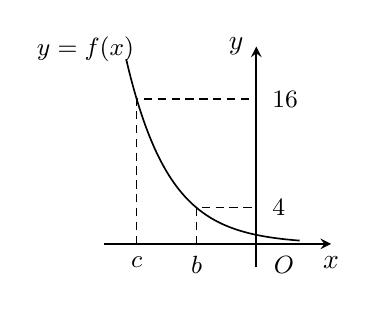
\begin{tikzpicture}[line width=0.6pt, x=0.38cm, y=0.115cm, >=stealth]
  \draw[densely dashed, line width=0.4pt] (-4,0) -- (-4,16) -- (0,16);
  \draw[densely dashed, line width=0.4pt] (-2,0) -- (-2,4) -- (0,4);
  \draw[->, line width=0.7pt] (-5.1,0) -- (2.5,0) node[below=1pt] {$x$};
  \draw[->, line width=0.7pt] (0,-2.6) -- (0,21.8) node[left=1pt] {$y$};
  \draw[domain=-4.35:1.45, samples=90, smooth] plot (\x, {pow(0.5,\x)});
  \node[anchor=west, font=\small] at (0.2,16) {$16$};
  \node[anchor=west, font=\small] at (0.2,4) {$4$};
  \node[anchor=north, font=\small] at (-4,-0.3) {$c$};
  \node[anchor=north, font=\small] at (-2,-0.3) {$b$};
  \node[anchor=north west, font=\small] at (0.25,-0.3) {$\pt{O}$};
  \node[anchor=south east, font=\small] at (-3.75,19.0) {$y=f(x)$};
\end{tikzpicture}
